\chapter{Analýza}\label{chapter:analyza}
% Hlavním cílem této bakalářské práce je implementovat návrh backendu podle návrhu a fragmentu implementace, které byly udělány v rámci předmětů BI-SP1 a BI-SP2 bakalářského studia vyučovaných na FIT ČVUT v akademickém roce 2018/2019 a 2019/2020. 

%TODO move commit footnote to reserse and git footnote
Tato kapitola se zabývá analýzou existujícího nárhu a současného stavu implementace. Pro jasné zajištěni verze aplikace, která bude předmětem analýzy této kapitoly, uvádím datům ukončení práce na projektu v rámci předmětu BI-SP2 -- 25. února 2020. Také pro možnost pohodlného vyhledání konkretní verze  (\url{https://gitlab.fit.cvut.cz/rozvody/be-springboot}), uvádím poslední \texttt{commit}\footnote{proces při kterém se uloží všechny udělané v rámci systému řízení verzí změny a zařadí se do historie změn} udělaný přes Git\footnote{ distribuovaný systém řízení verzí} v rámci tohoto předmětu: 
\begin{quote}
    \enquote{252b0288dbfe9942446b78fd452c0edce810a370}
\end{quote}

\section{Předmět BI-SP1}\label{analyza:navrh:sp1}
    % TODO REST footmote to first mention
    V rámci předměty BI-SP1 pracovalo sedm lidí včetně autora této práci. Tým měl za úkol analyzovat požadavky zákazníka a navrhnout implementaci aplikace. Během semestru tým provedl kompletní analýzu požadavku zákazníka. Především, tým navrhl scénáře použiti aplikace:
    \begin{itemize}
	   \item Přihlašování/Registrace;
	   \item Přihlašování/Registrace do rodiny;
	   \item Role v aplikace a jejich vytváření;
	   \item Nastavení pečovatelský dnů;
	   \item Kalendář;
	   \item Kniha potřeb dítěte;
	   \item Uchování účtenek;
	   \item Správa alimentů.
	\end{itemize}
    Potom byly navrženy diagram užití\footnote{popisuje chování systému z vnějšího pohledu} a diagram aktivit\footnote{zobrazuje jak objekty spolupracují}, podle kterých byly navrženy Wireframy\footnote{grafickém zobrazením hlavních prvků frontendové částí aplikace} a doménový model\footnote{náčrt základních entit systému a vztahů mezi nimi}. 
    
    Výsledný návrh aplikace se skládá ze dvou částí. Serverového backendu, který je předmětem této bakalářské práci a frontendové částí aplikace, kterou současně řeší kolega -- Martin Beran -- v rámci bakalářské prací. Frontendová část aplikace je Android aplikací. Backendová část je serverovým backendem, poskytujícím REST\footnote{Representational State Transfer} API pro Android aplikaci.

\section{Předmět BI-SP2}\label{analyza:navrh:sp2}
    %TODO gradle footnote to reserse and Spring footnote
    Cílem předmětu BI-SP2 byla implementace návrhu předmětu BI-SP2. Autor této práce pracoval v backendovém týmu a zároveň vystupoval v roli vedoucího backendového týmu.
    
    Pro vývoj backendove částí aplikace byl zvolen jazyk Kotlin, zmíněný v sekci \ref{resere:kotlin}, a framework Spring, zmíněný v sekci \ref{resere:j2ee}. Jako {buildovací system}\footnote{nástroj pro automatizaci sestavování programu} byl zvoleny nástroj Gradle. Podrobněji výsledky předmětu BI-SP2 budou probrány v sekci \ref{analyza:soucasnaImplementace}.
        
    
\section{Doménový model}\label{analyza:navrh:DomainModel}
    Hlavním zdrojem informace o výsledném návrhu serveru je doménový model. Kompletní doménový model se nachází v příloze \ref{dodatek:DomainModel}. Během implementace tým označoval entity, které jsou kompletně nebo částečně implementovány. Zelenou barvou jsou označeny třídy, které už jsou implementovány. Žlutou barvou jsou označeny třídy, které ještě nejsou implementovány. Také, jsou třídy označeny zároveň žlutou a zelenou barvou, což znamená, že třída je implementována jenom částečně. Taková situace se mohla nastat v případe, že implementace vyžadovala implementace jiné třídy, která ještě neexistovala. Tento doménový model má určité nedostatky podle požadavku frontedové části aplikace. Jako příklad takových nedostatků je možné uvést zbytečně komplikovaný návrh entity \texttt{Interval} (viz obrázek \ref{image:Interval1}). Podrobný popis problému bude uveden v sekci \ref{analyza:pozadavky-frontendu}.

\section{Analýza současného návrhu} \label{analyza:analyza navrhu}
    V této sekci budou podrobně popsány klíčové aspekty aplikace podle současného návrhu. Problémy a navržené změny těchto částí budou popsány v následujících sekcích.

    \subsection{Registrace a přihlášeni do systému}
        Aplikace je navržena takovým způsobem, že první uživatel, který má vytvořit svůj účet je jeden z rodičů. Pro registraci člověk potřebuje řadu povinných údajů:
        \begin{itemize}
	        \item \texttt{name} -- zvolené jméno se stává jeho implicitním jménem v systému.
	        \item \texttt{surname} -- zvolené příjmení se stává jeho implicitním příjmením v systému.
	        \item \texttt{email} -- zvolený email je identifikátorem uživatele v rámci systému.
	        \item \texttt{password} -- heslo pro autorizaci v systému.
        \end{itemize}
        Na základe těchto údajů se vytváří unikátní uživatel v rámci systému. V tento okamžik člověk není přihlášeny do žádné rodiny a nemá žádnou roli. Podrobněji role budou popsané v sekci \ref{analyza:bezpecnost:role}.
        % \begin{figure}\centering
	       % 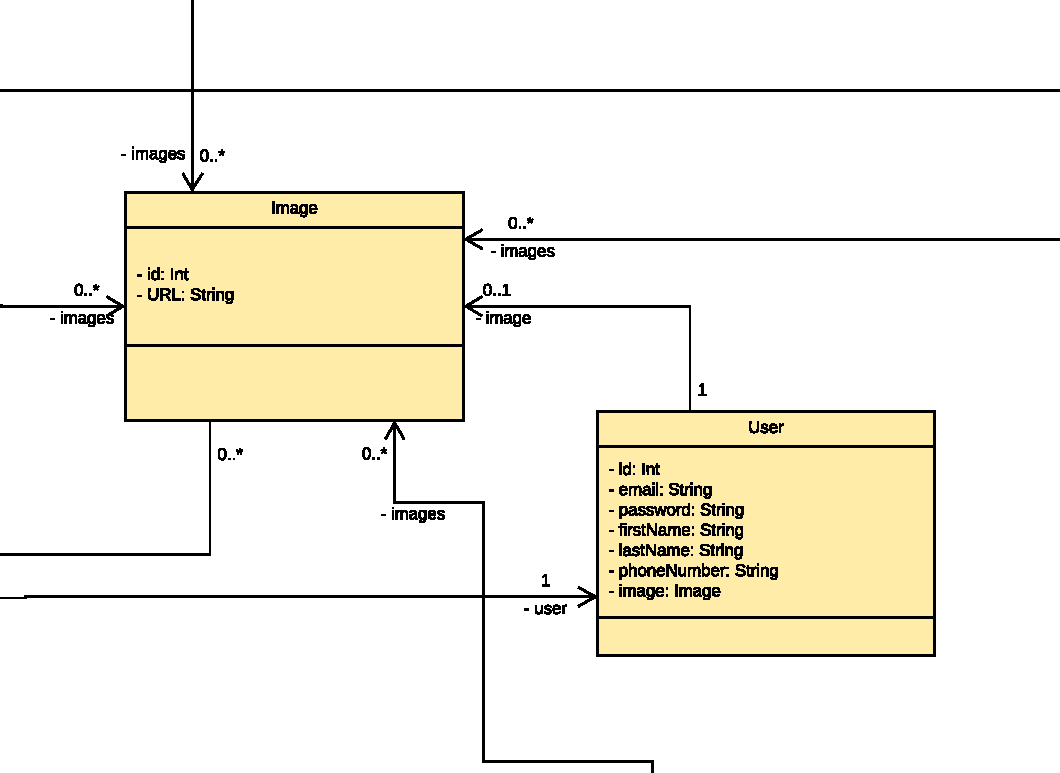
\includegraphics[width=0.7\textwidth]{pdfs/User-Image1}
	       % \caption[Návrh User-Image]{Vztah mezi třídami \texttt{User} a \texttt{Image} podle Doménového modelu z předmětu BI-SP2}\label{image:User-Image1}
        % \end{figure}
        
        Potom uživatel má možnost vytvořit rodinu nebo přihlásit se do již existující rodiny. Pro vytvoření nové rodiny, uživatel potřebuje zadat jméno rodiny a přidat členy rodiny. Autor této rodiny automaticky se stává jedním s rodičů této rodiny. Jinou možností je přihlásit se do rodiny, která již existuje. Podmínkou je existování pozvání do některé existující rodiny, což znamená, že přidat nového uživatele do rodiny může jenom člen této rodiny.V takovém případě uživatel už nemá možnost zvolit role v rámci rodiny. Role má být nastavena uživatelem, který vytvořil toto pozvání.

    \subsection{Kalendář}    
        Kalendář je hlavním zdrojem informaci pro celou rodinu a je společný pro všechny uživatele. Na něm jsou zobrazené zvýrazněné různými barvami pečovatelské dny obou rodičů. Členy rodiny mají možnost požádat o převzetí péče pro konkretní den nebo časový interval. Takový postup pomáhá rodině eliminovat situace, kdy několik členů rodiny najednou myslí, že je v konkretní den dítě v jejích péči nebo několik členu rodiny najednou říkají, že není to jejích den. Kromě pečovatelských dnů, kalendář také zobrazuje jednorázové a pravidelné události.
        
        \begin{figure}\centering
	        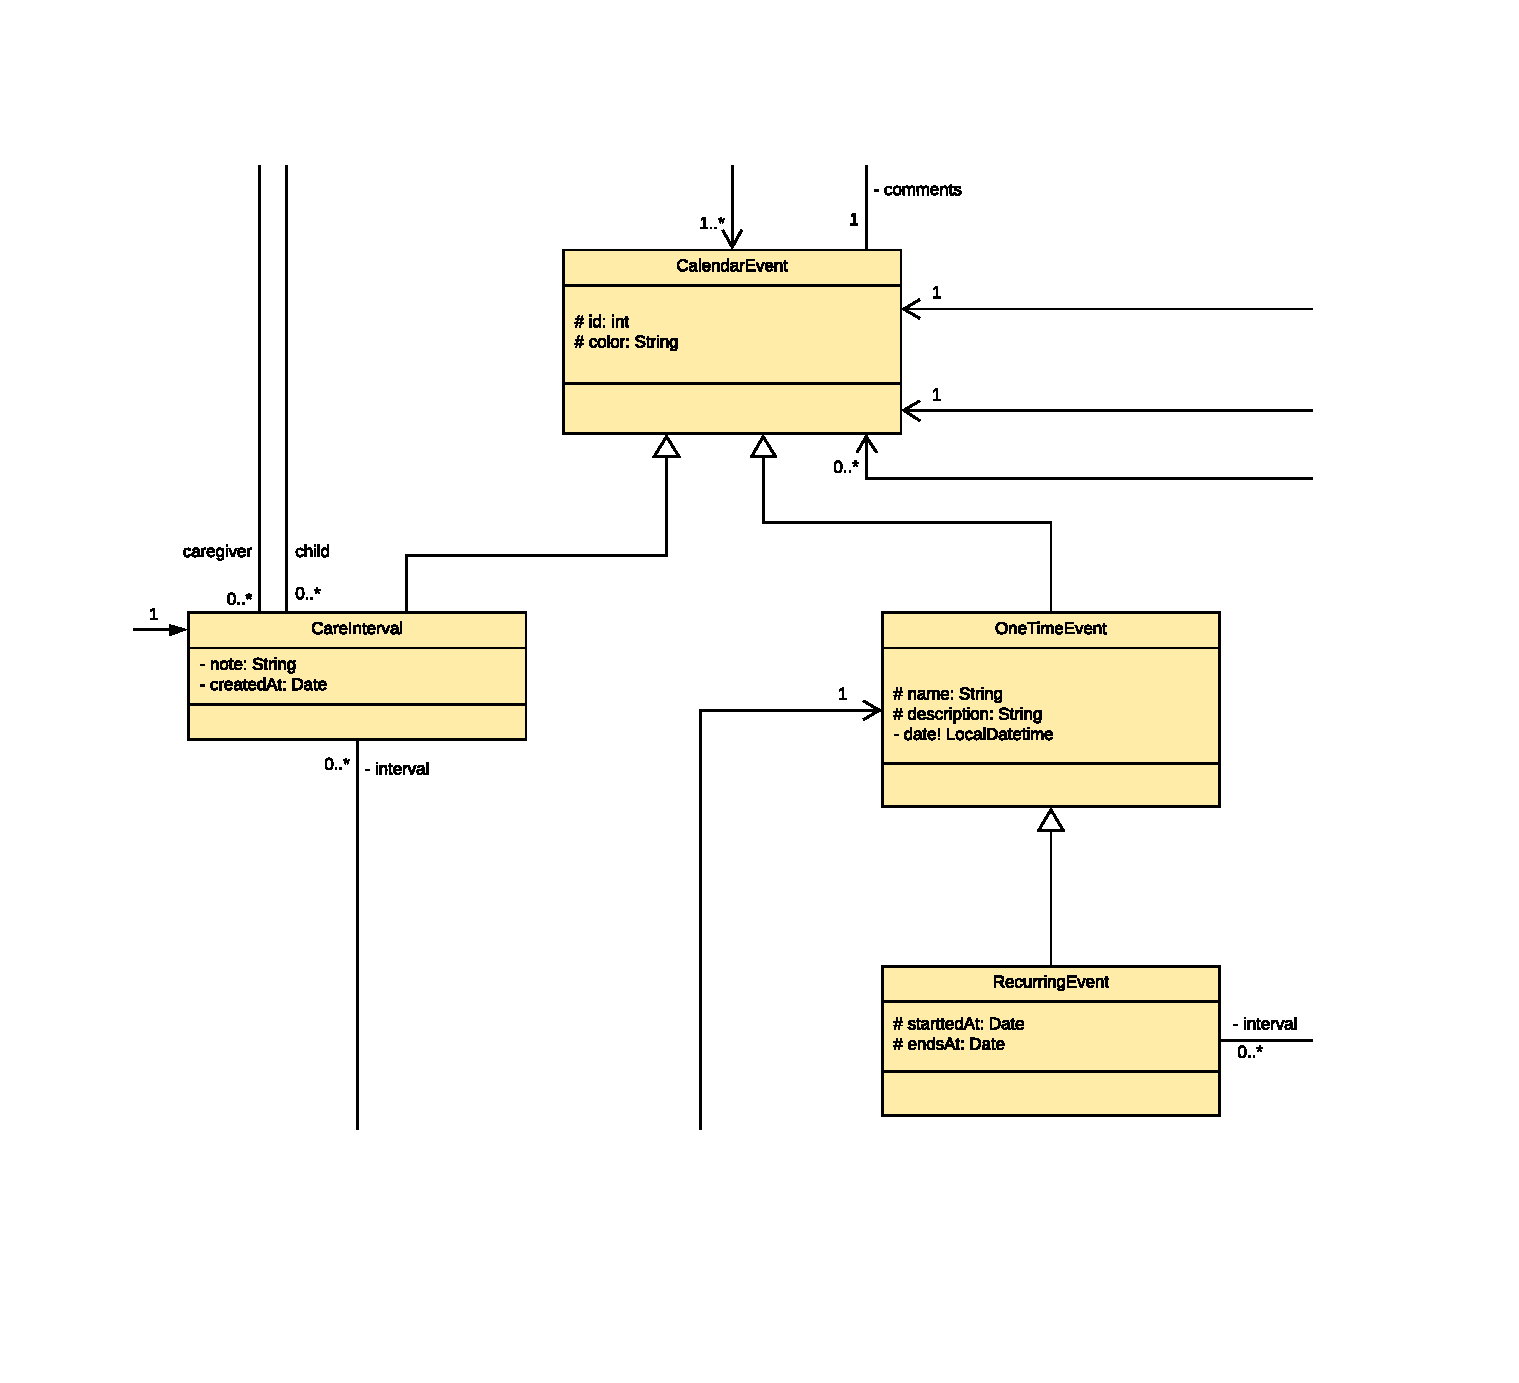
\includegraphics[width=1.0\textwidth]{pdfs/CalendarInfo1}
	        \caption[Současný návrh kalendáře]{Návrh kalendáře podle doménového modelu z předmětu BI-SP2}\label{image:calendar-info}
        \end{figure}
        Doménový model neobsahuje informaci o kalendáře, ale obsahuje entity reprezentující informaci, kterou kalendář bude zobrazovat (viz obrázek \ref{image:calendar-info}). Každý element, který bude zobrazen v kalendáři, je reprezentován stejnou entitou \texttt{CalendarEvent}. Entita obsahuje jenom informaci o barvě, kterou bude zobrazená v kalendáři, a závislost na entitu \texttt{Comment}. Za reprezentací pečovatelských dnů odpovídá entita \texttt{CareInterval}, která se dědí od entity \texttt{CalendarEvent}. Za reprezentaci jednorázových a opakujících se události odpovídají entity \texttt{OneTimeEvent} a \texttt{RecurringEvent}, kde \texttt{RecurringEvent} se dědí od \texttt{OneTimeEvent}.
        
        % Současný návrh kalendáře nepokrývá všechny scénáře použití. Podrobný popis problémů a navržené změny budou uvedeny v sekci \ref{analyza:kalendar}. 
        
        % Kromě dlouhodobých nastavení pečovatelských dnu, kalendář může zobrazovat i jednorázové změny, které mohou vidět všechny členy rodiny. 
    \subsection{Alimenty}
        \begin{figure}\centering
	        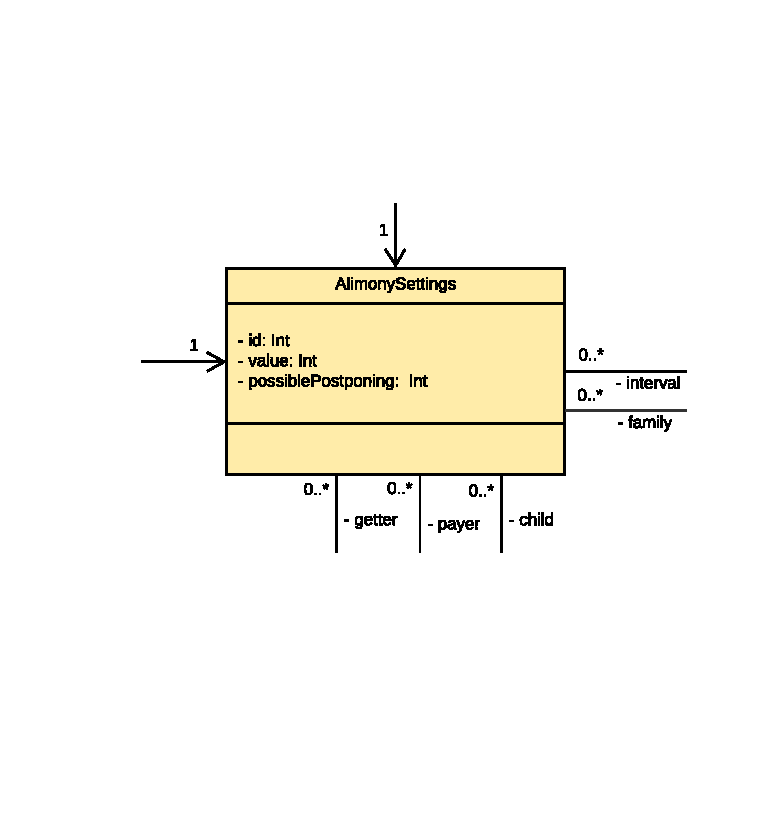
\includegraphics[width=0.5\textwidth]{pdfs/AlimonySettings1}
	        \caption[Návrh AlimonySettings]{Návrh třídy \texttt{AlimonySettings} podle Doménového modelu z předmětu BI-SP2}\label{image:AlimonySettings1}
        \end{figure}
        \begin{figure}\centering
	        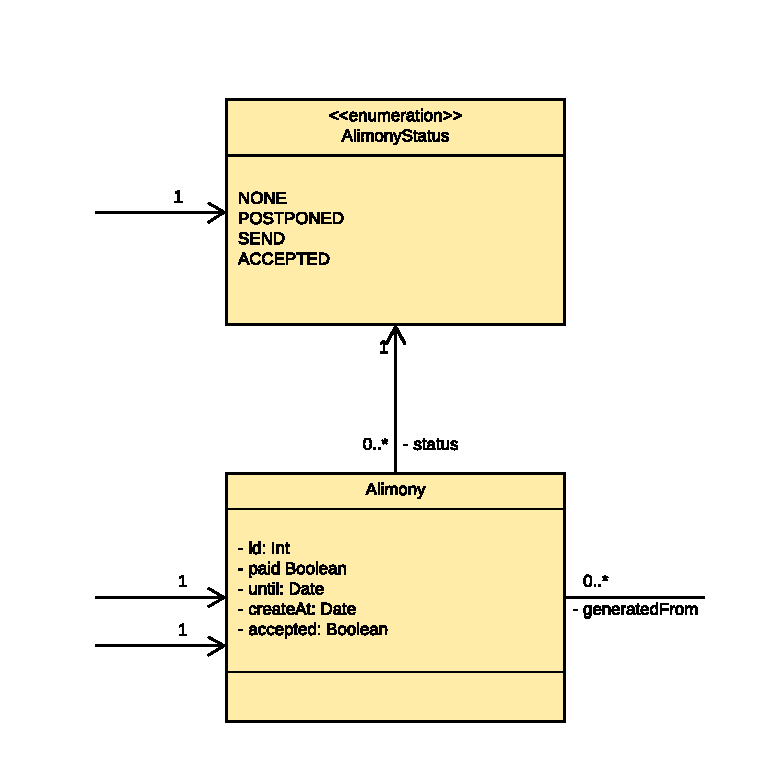
\includegraphics[width=0.5\textwidth]{pdfs/Alimony1}
	        \caption[Návrh Alimony]{Návrh třídy \texttt{Alimony} podle Doménového modelu z předmětu BI-SP2}\label{image:Alimony1}
        \end{figure}
        Důležitou částí aplikace je správa alimentů, které má pravidelně uhrazovat jeden z rodičů. Tento proces byl rozdělen do dvou částí. První částí je dlouhodobé nastavení alimentů (viz obrázek \ref{image:AlimonySettings1}). Druhou částí jsou samotné alimenty (viz obrázek \ref{image:Alimony1}), které se generuje na základě dlouhodobých nastavení. Jedna rodina může mít zároveň několik nastavení v případě, že jedna rodina má několik dětí nebo chce rozdělit alimenty do logických částí.
        
        Každá instance alimentů má stav, který se postupně mění. V moment vytvoření instance má stav \verb|NONE|. Po odesílání alimentů druhému rodiči, stav se mění na \verb|SEND|. Potom druhý rodič má potvrdit, že alimenty přijal, a tím změnit stav na \verb|ACCEPTED|. Také se může nastat situace, kdy rodič nemá možnost odeslat alimenty včas, což se může nastat z různých důvodů. V takovém případě stav instanci se mění na \verb|POSTPONED|.
    
    \subsection{Kniha potřeb dítěte}\label{analyza:navrh:need}
        \begin{figure}\centering
	        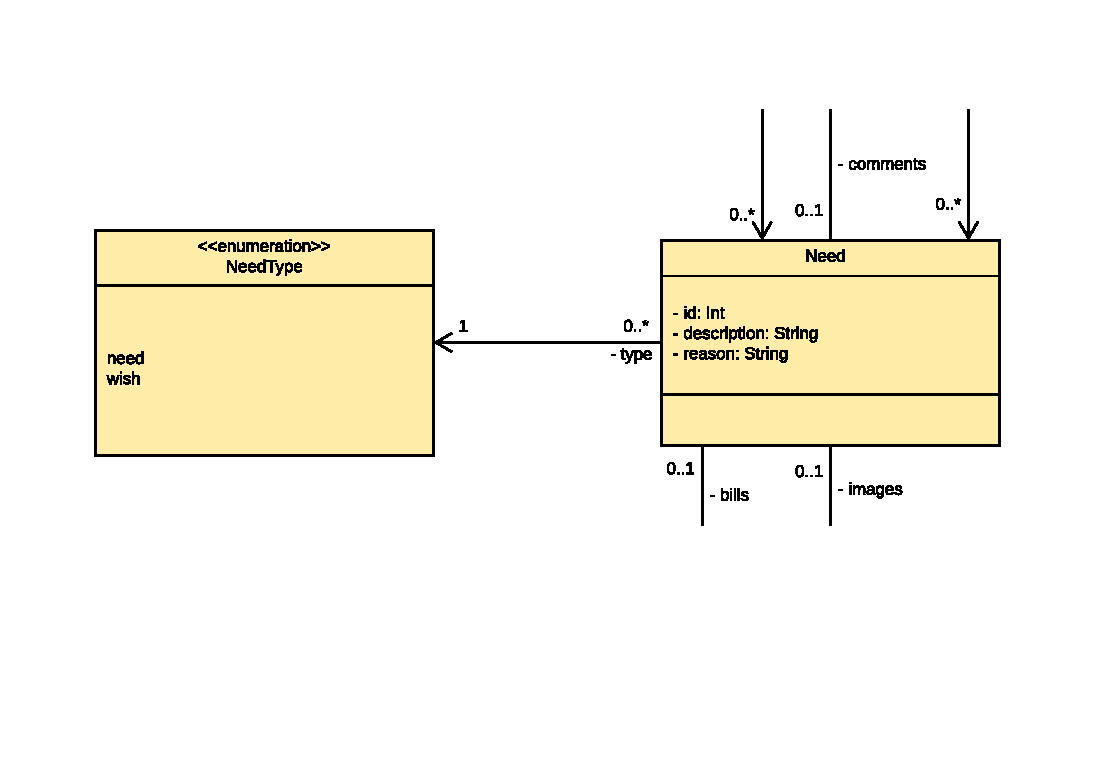
\includegraphics[width=0.5\textwidth]{pdfs/Need1}
	        \caption[Návrh \texttt{Need}]{Návrh entity \texttt{Need} podle doménového modelu z předmětu BI-SP2}\label{image:Need1}
        \end{figure}
        Jedním s populárních problémů, které vznikají během procesu rozvodu, je nakupování příliš drahých dárku o kterých nevědí ostatní členy rodiny. Jako příklad je možné uvést nakupování bot pro dítěte. Jeden s rodičů může chtít \enquote{koupit lásku dítěte} a koupit několikrát dražší boty než dítě opravdu potřebuje. Kniha potřeb dítěte (viz obrázek \ref{image:Need1}) je zaměřena na překonání takových situací.
        
        \begin{figure}\centering
	        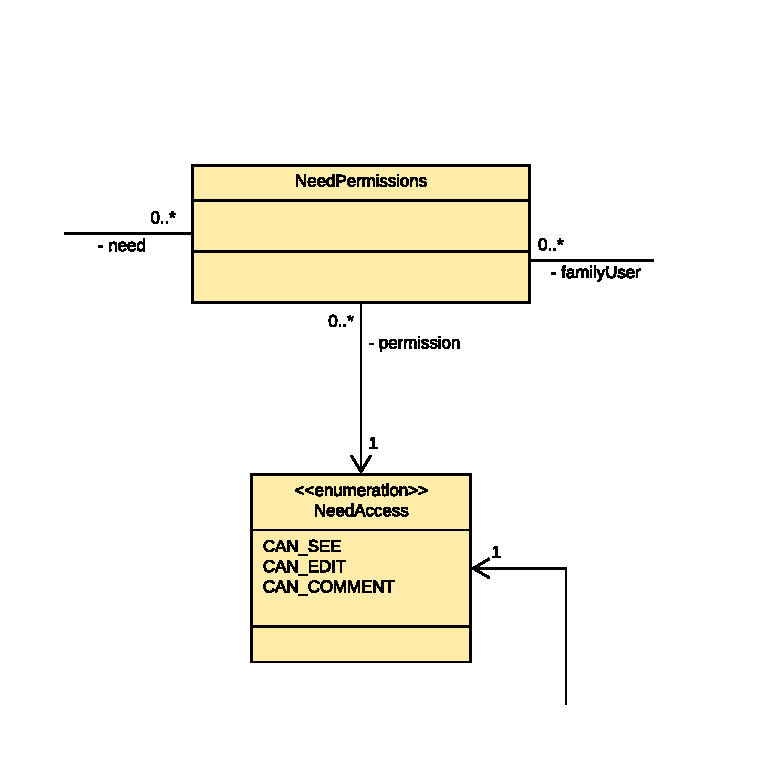
\includegraphics[width=0.7\textwidth]{pdfs/NeedPermissions1}
	        \caption[Návrh \texttt{NeedPermissions}]{Návrh entity \texttt{NeedPermissions} podle doménového modelu z předmětu BI-SP2}\label{image:NeedPermissions1}
        \end{figure}
        Potřeba může být typu \texttt{need} a \texttt{wish}. Podle současného návrhu je rozdíl mezi typy pouze pro informační účely. Každé instance entity \verb|Need| patři instance entity \verb|NeedPermission| (viz obrázek \ref{image:NeedPermissions1}), která definuje přístupová práva pro jednotlivé členy rodiny. V případě, že uživatel nemá žádné z přístupových práv, potřeba se nevyskytuje v jeho seznamu potřeb dítěte. Toto pravidlo se netýká jenom rodičů, které mají přistup ke všem potřebám automaticky.
       
       Potřeba obsahuje následující informaci:
        \begin{itemize}
            \item \texttt{description} -- popis potřeby.
            \item \texttt{reason} -- příčina proč dítě tohle potřebuje.
            \item \texttt{images} -- obrázky věcí, kterou dítě potřebuje.
            \item \texttt{bills} -- účtenky v případě, že někdo z rodičů splnil potřebu.
            \item \texttt{comments} -- komentáře členu rodiny včetně dítěte.
        \end{itemize}
    
    \subsection{Účtenky}
        \begin{figure}\centering
	        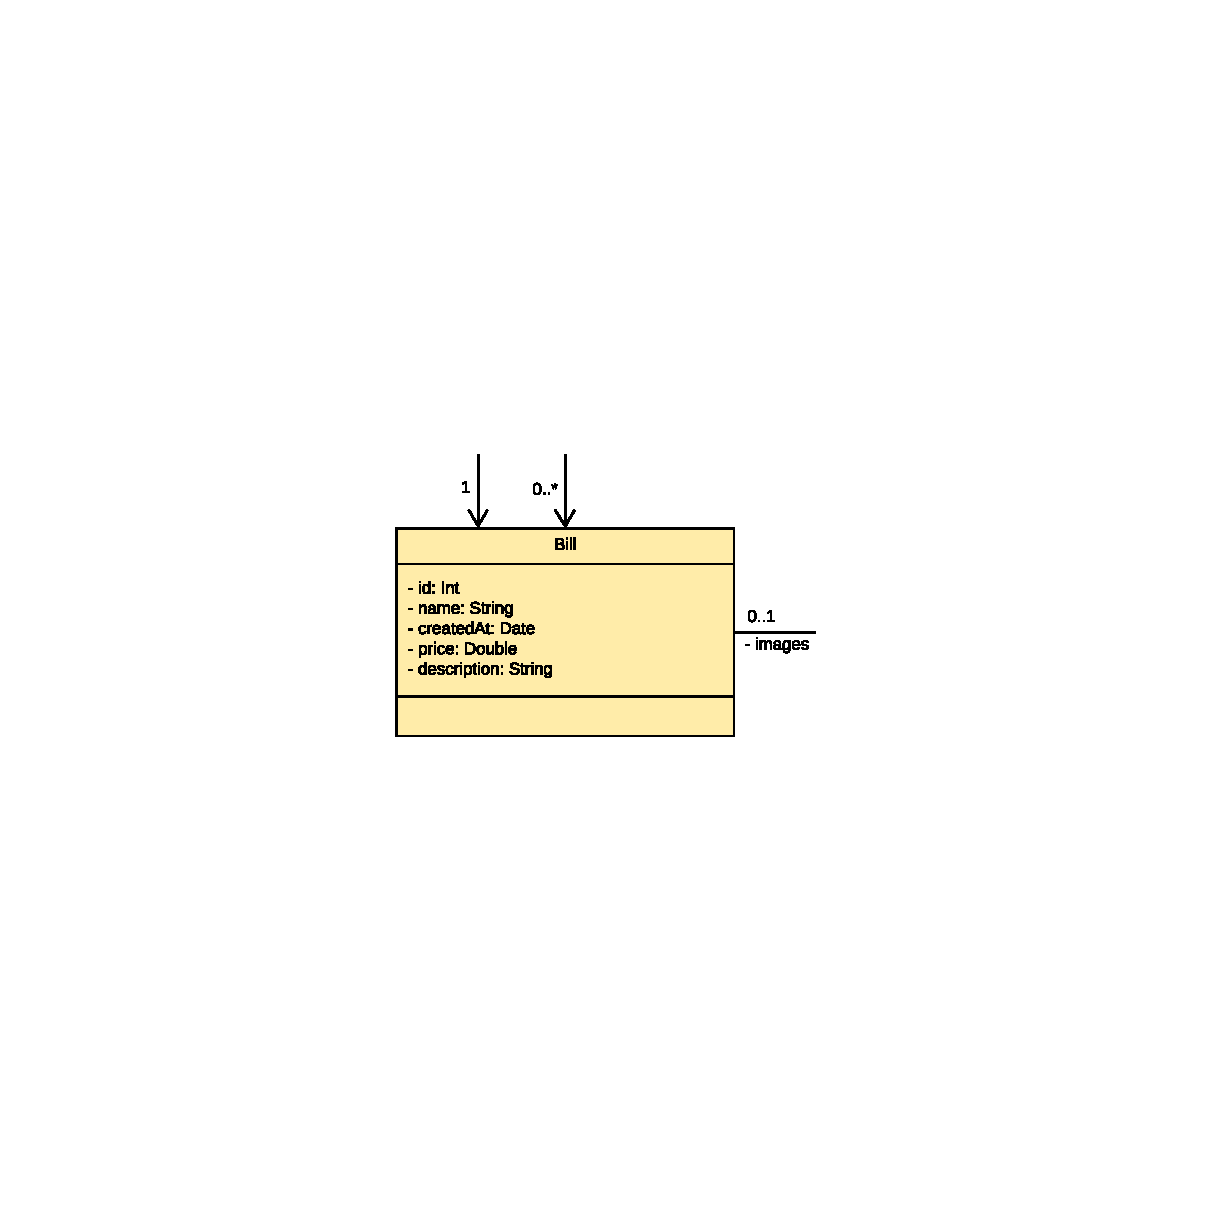
\includegraphics[width=0.5\textwidth]{pdfs/Bill1}
	        \caption[Návrh entity \texttt{Bill}]{Návrh entity \texttt{Bill} podle doménového modelu z předmětu BI-SP2}\label{image:bill1}
        \end{figure}
        V sekci \ref{analyza:navrh:need} už bylo zmíněno, že je potřeba řešit problém nakupování dárku pro dítěte, ale kniha potřeb dítěte řeší tenhle problém jenom částečně. Nikdo nezabraní uživateli uvést v popisu splněného požadavku nebo potřeby neplatné údaje, proto byla zavedena možnost přidání účtenky (viz obrázek \ref{image:bill1}). Tato entita, kromě údajů o nakoupeném zboží, umožňuje přidání fotografií potvrzujících platnost uvedených údajů.
    
    \subsection{Požadavky na změny}
        Každý člen rodiny může udělat určité změny v rámci rodiny. Například nastavit přezdívku pro konkretního uživatel nebo přidat fotografii do události v kalendáři. Každá taková změna je důležitá, ale jsou změny, které by měly být kontrolovány rodiči. Pro zaručení kontroly byly zavedeny požadavky na změny pro některé změny v rámci rodiny:
        \begin{itemize}
            \item \texttt{AlimonySettingRequest} -- požadavek na změnu nastavení alimentů, který může být vytvořen jedním z rodičů.
            \item \texttt{AlimonyChangeRequest} -- požadavek na změnu stavu instance alimentů, který může být vytvořen jedním z rodců
            \item \texttt{OneTimeEventRequest} -- požadavek na vytvoření jednorázové události v kalendáři, který může být vytvořen libovolným cleném rodiny,
            \item \texttt{OneTimeEventChangeRequest} -- požadavek na změnu již existující události v kalendáři, který může být vytvořen libovolným členém rodiny.
            \item \texttt{ChildItemRequest} -- požadavek na změnu nastavení pečovatelských dnů, který může vytvořit libovolný člen rodiny. Změna může být, jak jednorázová, tak i dlouhodobá.
        \end{itemize}
        \begin{figure}\centering
	        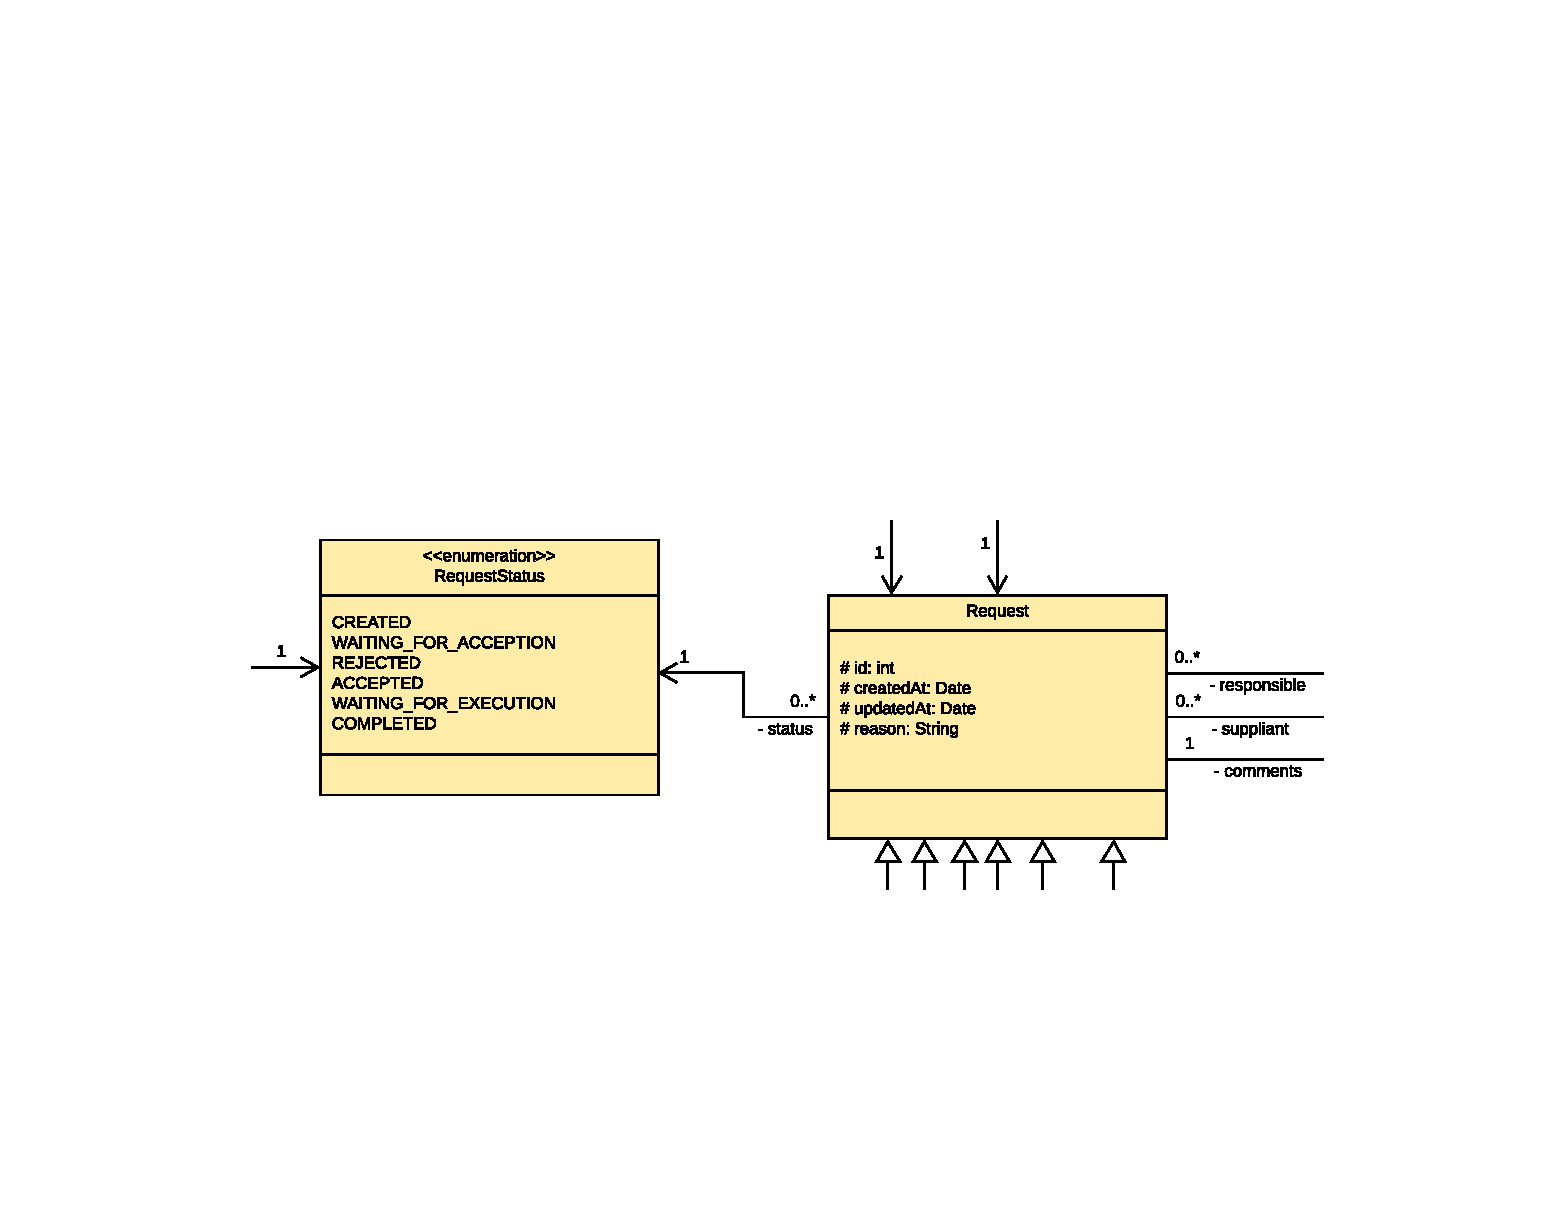
\includegraphics[width=0.7\textwidth]{pdfs/Abstr-Requrest1}
	        \caption[Návrh abstraktní entity \texttt{Request}]{Návrh abstraktní entity \texttt{Request} podle doménového modelu z předmětu BI-SP2}\label{image:abstr-request1}
        \end{figure}
        Každá entita požadavku je zděděna od společné abstraktní entity obsahující základní informaci o požadavku (viz obrázek \ref{image:abstr-request1}). Mezi základní informacemi patří datum vytvoření, datum poslední změny, příčina a také aktuální status požadavku.
        
        Status požadavku reprezentují jeho životní cyklus. Při vytvoření každý požadavek má stejný status -- \verb|CREATED|. Po zveřejnění, požadavek má status \verb|WAITING_FOR_ACCEPTING|. Po schváleni, status se mění na \verb|ACCEPTED| nebo na \verb|WAITING_FOR_EXECUTION| v případě, že změna se akceptována, ale ještě není uplatněna. Také může nastat případ, že požadavek byl zamítnut, potom status se mění na \verb|REFECTED|. V okamžik, kdy požadavek je schválen nebo se čeká m uplatnění, už není možné měnit položky tohoto záznamu. Právo na schválení nebo zamítnutí požadavků mají jenom rodiče. Požadavky, které byly vytvořeny jedním z rodičů, mají být potvrzeny druhým rodičem. Ostatní požadavky musí být potvrzeny oběma rodiči.
    
    \subsection{Historie změn}
        Podle požadavků zákazníka, všechny změny v rámci rodiny by měly být zaznamenány. Proto byly zavedeny entity, které kopírují všechny položky entit a přidávají datum vytvoření záznamu a odkaz do patřičné entity v případě, že táto příslušná entita byla aktualizována. Takové entity jsou zavedeny jenom pro důležité části aplikace, které se mohou měnit uživatelem:
        \begin{itemize}
            \item \texttt{CalendarEventHistory}.
            \item \texttt{BillHistory}.
            \item \texttt{AlimonyHistory}.
            \item \texttt{AlimonySettingsHistory}.
            \item \texttt{RequestHistory}.
        \end{itemize}
        Všechny typy historie jsou zděděny od stejné entity -- \texttt{History}. Tato entita obsahuje základní údaje pro libovolný typ historie: ID\footnote{identifikátor} a datum vytvoření záznamu. 
     
\section{Analýza současné implementace}\label{analyza:soucasnaImplementace}
    \begin{figure}\centering
	   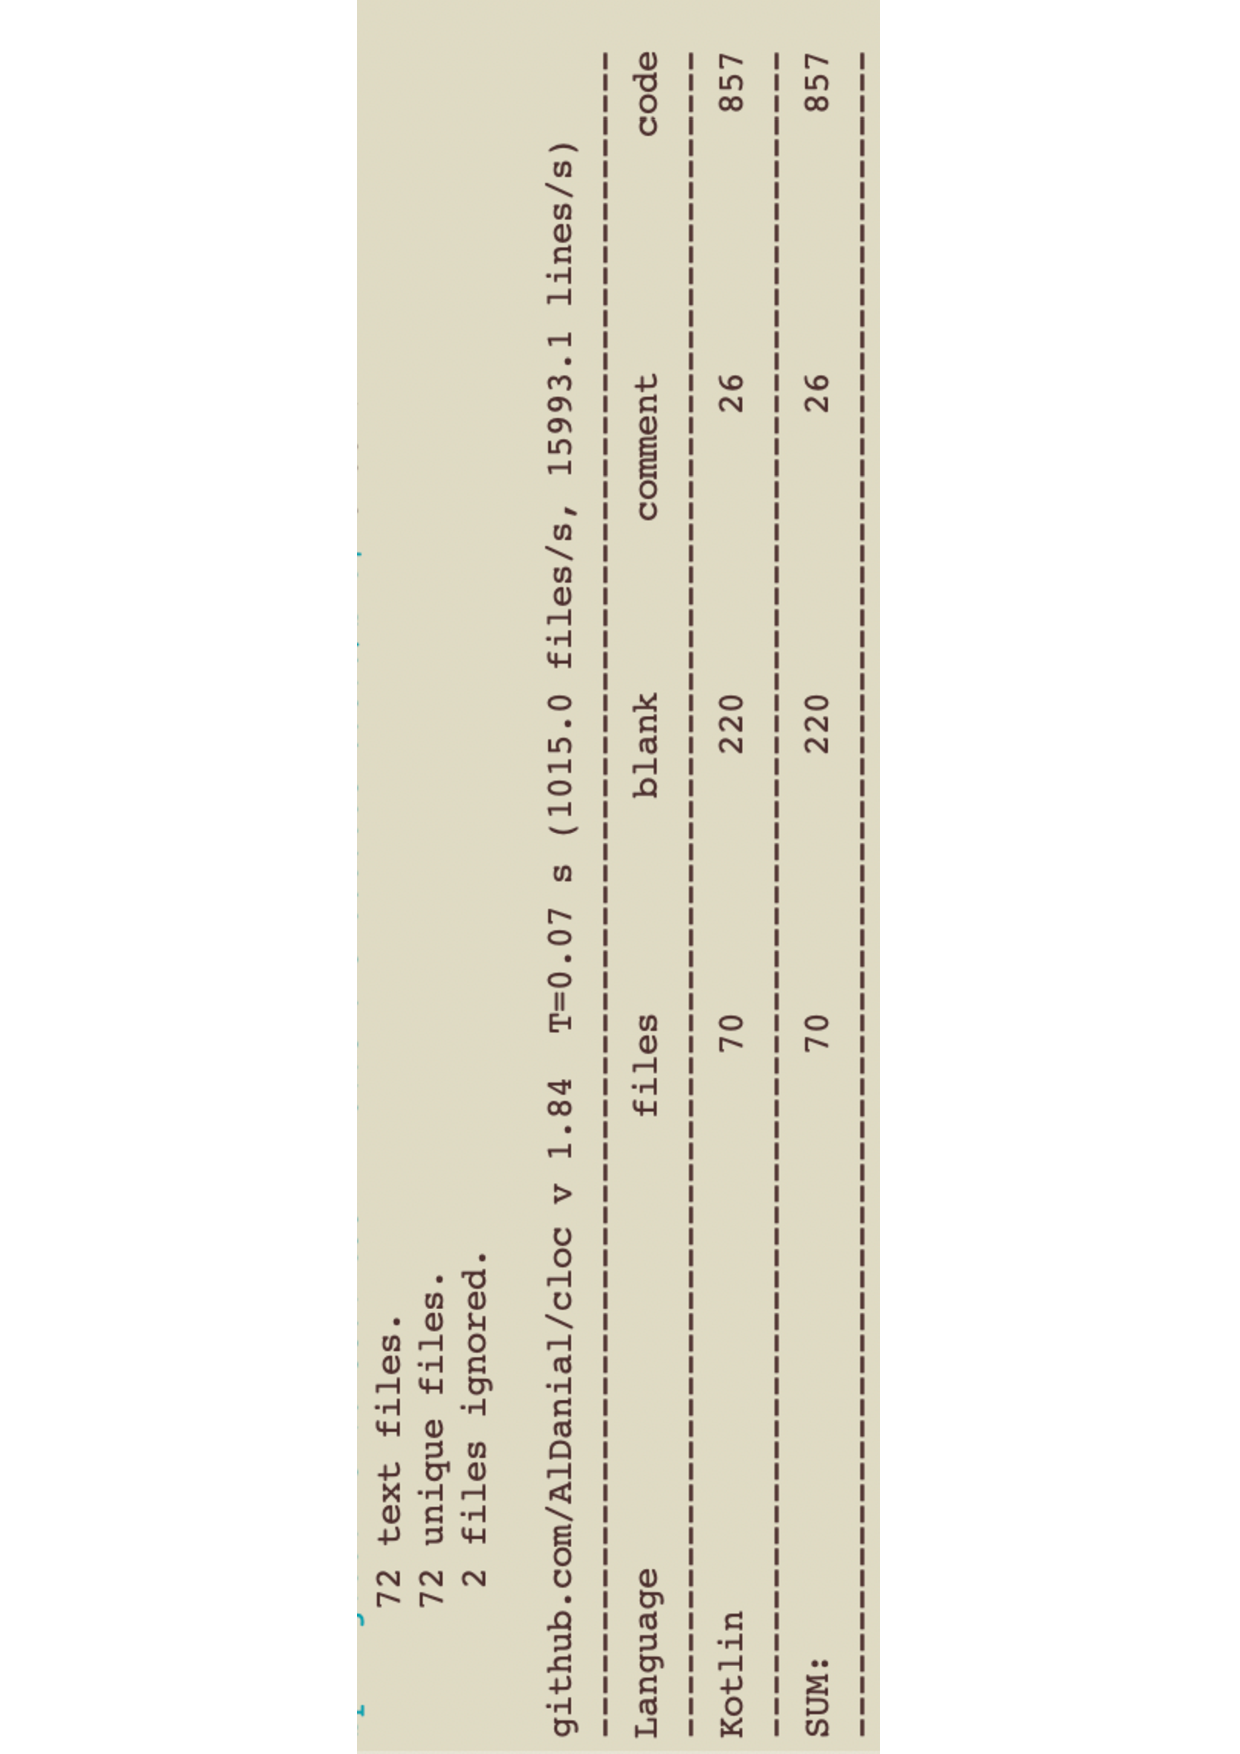
\includegraphics[angle=-90, width=0.7\textwidth]{pdfs/Cloc1}
	   \caption[Počet řádků kódu před začátkem práce]{Počet řádků kódu před začátkem práce}\label{image:cloc1}
    \end{figure}
     V této sekci bude stručně popsán současný stav implementace. Současná implementace obsahuje 69 souborů a 845 řádek kódů (viz~obrázek~\ref{image:cloc1}), které byly vytvořeny a napsány členy týmu. Za účelem zvětšení přesnosti analýzy byl zvolen nástroj pro analýzu počtu řádek kódu - CLOC (viz sekci \ref{reserse:cloc}). Implementace částečné pokrývá doménový model zmíněný v sekci. \ref{analyza:navrh:DomainModel}.
        
    \subsection{Implementované třídy}
        Seznam implementovaných entit:
        \begin{itemize}
            \item \texttt{AlimonyStatus}
            \item \texttt{Bill}
            \item \texttt{CalendarEvent}
            \item \texttt{OneTimeEvent}
            \item \texttt{Comment}
            \item \texttt{FamilyMember} - částečně
            \item \texttt{History}
            \item \texttt{IntervalType}
            \item \texttt{NWeekInterval}
            \item \texttt{WeekInterval}
            \item \texttt{NeedAccess}
            \item \texttt{NeedType}
            \item \texttt{NeedType}
            \item \texttt{AbstractPermissions}
            \item \texttt{Permissions}
            \item \texttt{RequestStatus}
            \item \texttt{User}
        \end{itemize}
        
        Byl přidán \texttt{controller}\footnote{vrstva controlleru zajišťuje REST API komunikaci, překládá výjimky na HTTP kóda zajišťuje omezení pro jednotlivých uživatelů} pro testování, zda aplikace běží, který je namapován\footnote{přidání konkrétnímu controlleru adresy pomocí anotací frameworku Spring, která se zadává jako URI při odesílaní požadavků na Server} na cestu \enquote{/}. Také, byla přidaná třída, která obsahuje nápovědy pro ostatní \texttt{controllery} ohledně zachycování chyb. Tato třída byla zavedena za účelem poskytování uživateli jenom korektně formátovanou informaci  a filtrování zbytečné informace pro koncového uživatele (viz tabulku \ref{tab:excpetion-handler1}). 
        \begin{table}\centering
	    \caption[Exception handler]{Ukázka \texttt{Exception handler} podle návrhu BI-SP2}\label{tab:excpetion-handler1}
	    \begin{tabular}{|l|c|c|c|}\hline
		  Typ chyby		& HTTP status		& zprava	& URL	\tabularnewline \hline \hline
		  \texttt{Illegal Access}	& 401	& původní zprava chyby		& původní cesta     \tabularnewline \hline
		  \texttt{Illegal Argument}	& 400	& původní zprava chyby		& původní cesta     \tabularnewline \hline
		  \texttt{Null Pointer}	& 500	& původní zprava chyby		& původní cesta     \tabularnewline \hline
		  \texttt{No Such Element}	& 404	& nic		& nic     \tabularnewline \hline
	    \end{tabular}
        \end{table}
    
    \subsection{Dokumentace API}
        Bylo provedeno nastavení frameworku Swagger pro dokumentace API (viz obrázek \ref{code:swagger-configuration}). Podrobněji framework Swagger byl popsán v sekci \ref{resere:dokumentace}.
        \begin{figure}
        \begin{minted}
        [frame=lines,
        framesep=2mm,
        baselinestretch=1.2,
        fontsize=\footnotesize,
        linenos]{java}
@Configuration
@EnableSwagger2
class SwaggerConfig {
@Bean
fun api(): Docket {
    return Docket(DocumentationType.SWAGGER_2)
        .select()
        .apis(RequestHandlerSelectors.any())
        .paths(PathSelectors.any())
        .build()
    }
}
        \end{minted}
        \caption{Ukázka nastavení frameworku Swagger}\label{code:swagger-configuration}
        \end{figure}
    
    \subsection{Profily}\label{analyza:soucasnaImplementace:profily}
    %spring profiles: https://docs.spring.io/spring-boot/docs/current/reference/html/spring-boot-features.html#boot-features-profiles
    %applicatioon peoperties: https://docs.spring.io/spring-boot/docs/current/reference/html/spring-boot-features.html#boot-features-external-config-application-property-files
        Framework Spring poskytuje možnost rozdělit implementaci do logických bloků, které budou existovat jenom v konkrétních profilech\cite{spring-profile}. Implicitně všechny komponenty nezávisle na aktuálních profilech. Pro zavedení profilů pro konkretní komponentu je potřeba ji označit anotací \texttt{Profile}. V závorkách vedle anotací je potřeba přidat seznam profilu, ve kterých tato komponenta bude existovat. Konfigurace aktuálně zapnutých profilů se provádí pomocí souboru \texttt{application.properties}, který definuje proměnné pro prostředí aplikace. Soubor se nachází ve složce s cestou \enquote{be-springboot/src/main/resources}.
    
        Každý profil také může obsahovat vlastní konfigurační soubor, který definuje všechny nutné proměnné. Soubor má byt zadán ve formátu \texttt{application-\{profile\}.properties}, kde \texttt{profile} je názvem profilu kterému patří tento soubor. Současný návrh aplikace obsahuje dva konfiguračních souboru.
    
        První konfigurační soubor obsahuje implicitní proměnné pro prostředí aplikace. Aktuálně soubor má jenom definici aktuálního profilu aplikace. 
    
        Druhý konfigurační soubor patří profilu \texttt{development}. Tento profil je určen pro pohodlný proces vývoje aplikace. Soubor obsahuje konfiguraci databáze a konfiguraci žurnálu aplikace. Podrobněji použita databáze pude popsána v sekci \ref{analyza:soucasnaImplementace:databaze}.
        
    \subsection{Databáze}\label{analyza:soucasnaImplementace:databaze}
        Pro proce vývoje byla zvolena relační databáze H2. Zvolená databáze umožňuje vytvářet tabulky při každém zapuštěni aplikace přímo v pamětí aplikace. Podrobněji tato databáze a její princip fungování byly popsány v sekci \ref{resere:databaze}.
    
\section{Analýza požadavku frontendu na změny}\label{analyza:pozadavky-frontendu}
    V rámci předmětu BI-SP2 současně s implementací backendové částí aplikace, probíhala implementace forntendové částí aplikace, která je reprezentovaná Android aplikací. Během vývoje frotnendové částí aplikace byly zjištěny nedostatky, které zbytečně komplikují implementaci, jak backendu, tak i frontendu.
    
    \subsection{Interval}
        Prvním takovým příkladem je návrh intervalu \ref{image:Interval1}, které jsou široce využívány v projektu. Návrh řešení tohoto problému bude popsán v sekci \ref{navrh:upravy}. tady bude popsán jenom problém samotný. Entita \texttt{Interval} reprezentuje časové rozmezí pro pečovatelské dny, opakované události, nastavení alimentů a navazující na ně požadavky na změny a historické záznamy.
            
        Jádro problému je v tom, že entita je navržena pomoci generalizace, neboli dědičnosti z hlediska implementace. Takový návrh dává možnost vytvořit konkretní typ intervalu pomocí zvolení odpovídající třídy, ale na druhou stranu působí komplikace při implementace a nepokrývá všechny možné případy potřebných intervalu. Například, není možné sestavit interval, který se bude opakovat každý poslední den měsíce. Pokud by jsme chtěli se držet se aktuální implementaci a zároveň pokryt všechny možné případy, ztratili bychom přehlednost zvolení správné třídy při vytváření instance \texttt{Intervalu}.
            
        Dalším problémem \texttt{Intervalu} je provázanost s pečovatelskými dny. Podle návrhu frontendové částí se bylo zjištěno, že pečovatelské dny nepotřebují komplikované nastavení a zároveň bych potřebovali mít odkazy na konkretního rodiče, který je zodpovědný za dítěte v tento den nebo časový úsek.
    
    \subsection{Alimenty}
        Druhou úpravou návrhu backendu, kterou potřebuje frontend, se tyká entity \texttt{ALimony}.
        Tato entita reprezentuje alimenty, které jeden rodič má posílat druhému rodiče. Jedna instance se odpovídá alimentům za jeden měsíc. Současný návrh popisuje návrh entity a její navázanost na entitu \texttt{AlimonySettings}(viz obrázek \ref{image:aliomny-draft1}), která definuje dlouhodobou konfiguraci, na základě které se vytváří jednotlivé instance alimentů. Nastavení alimentů se platí v rámci jedné rodiny. V případě potřeby, rodiče mají možnost rozdělit alimenty do několika nastavení. 
        
        Hlavní problém je v tom, že instance alimentů by se měly vytvářet nezávisle na frontendové části aplikace. Podrobně návrh řešení problému bude popsán v sekci \ref{navrh:upravy:alimenty}.
        
        Dodatečným požadavkem frontendového týmu se týká entity \texttt{Alimony} samotné. Za účelem zjednoduďení návrhu frontendové části je potřeba přidat závislost na entitu \texttt{Family}. % V takovém pŕípade aplikace může ihned po nalazení novych alimentu rict uZivateli ktere rodine patri tyto alimenty.
        \begin{figure}\centering
	        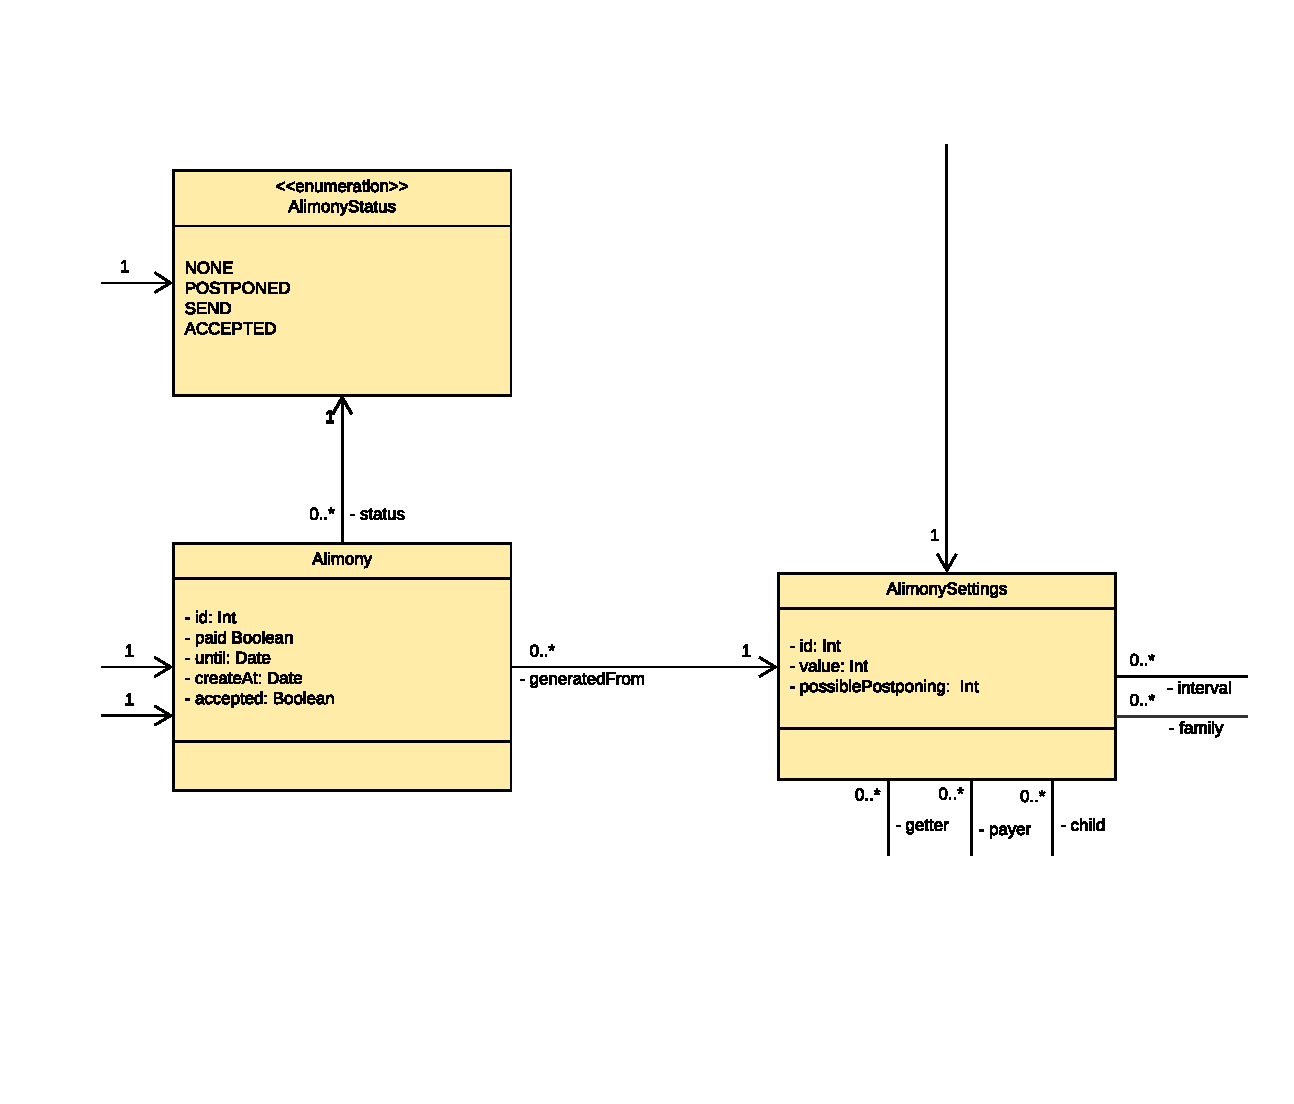
\includegraphics[width=0.7\textwidth]{pdfs/AlimonyDraft1}
	        \caption[Návrh \texttt{Alimony} a \texttt{AlimonySettings}]{Návrh entit \texttt{Alimony} a \texttt{AlimonySettings} podle Doménového modelu z předmětu BI-SP2}\label{image:aliomny-draft1}
        \end{figure}
        
        \subsection{Pečovatelské dny}\label{analyza:pozadavky:caredays}
            Než se zanořit do podrobného popisu problému, je potřeba popsat účel této entity a její využiti backendém a frontendém. Tato entita reprezentuje jednorázový interval nebo opakující interval pečovatelských jednoho z rodičů nebo libovolného jiného člena rodiny. Každý člen rodinu má vlastní barvou, která se využívá pro označování pečovatelských dnů v kalendáři. Tato entita se používá za dvěma účely. První a nejdůležitější účel je nastavení pečovatelských dnů pro rodiče. Nastavení musí pokrývat všechny dny kalendáře. Dítě by nemělo mít ve svém kalendáři den, který není označen žádnou barvou zároveň by neměly vznikat konflikty. Druhým účelem jsou jednorázové změny pečovatelských dnů. Tyto změny jsou vyžadovány pro případy, kdy dlouhodobé nastavení kalendáře neplatí. Příkladem může být výlet dítěte k babičce a dědečkovi. Během tohoto časového intervalu rodiče nejsou zodpovědné za dítěte, proto je potřeba uvést jednorázovou změny do kalendáře, která zaznamená tuto situaci 
            
            \begin{figure}\centering
	            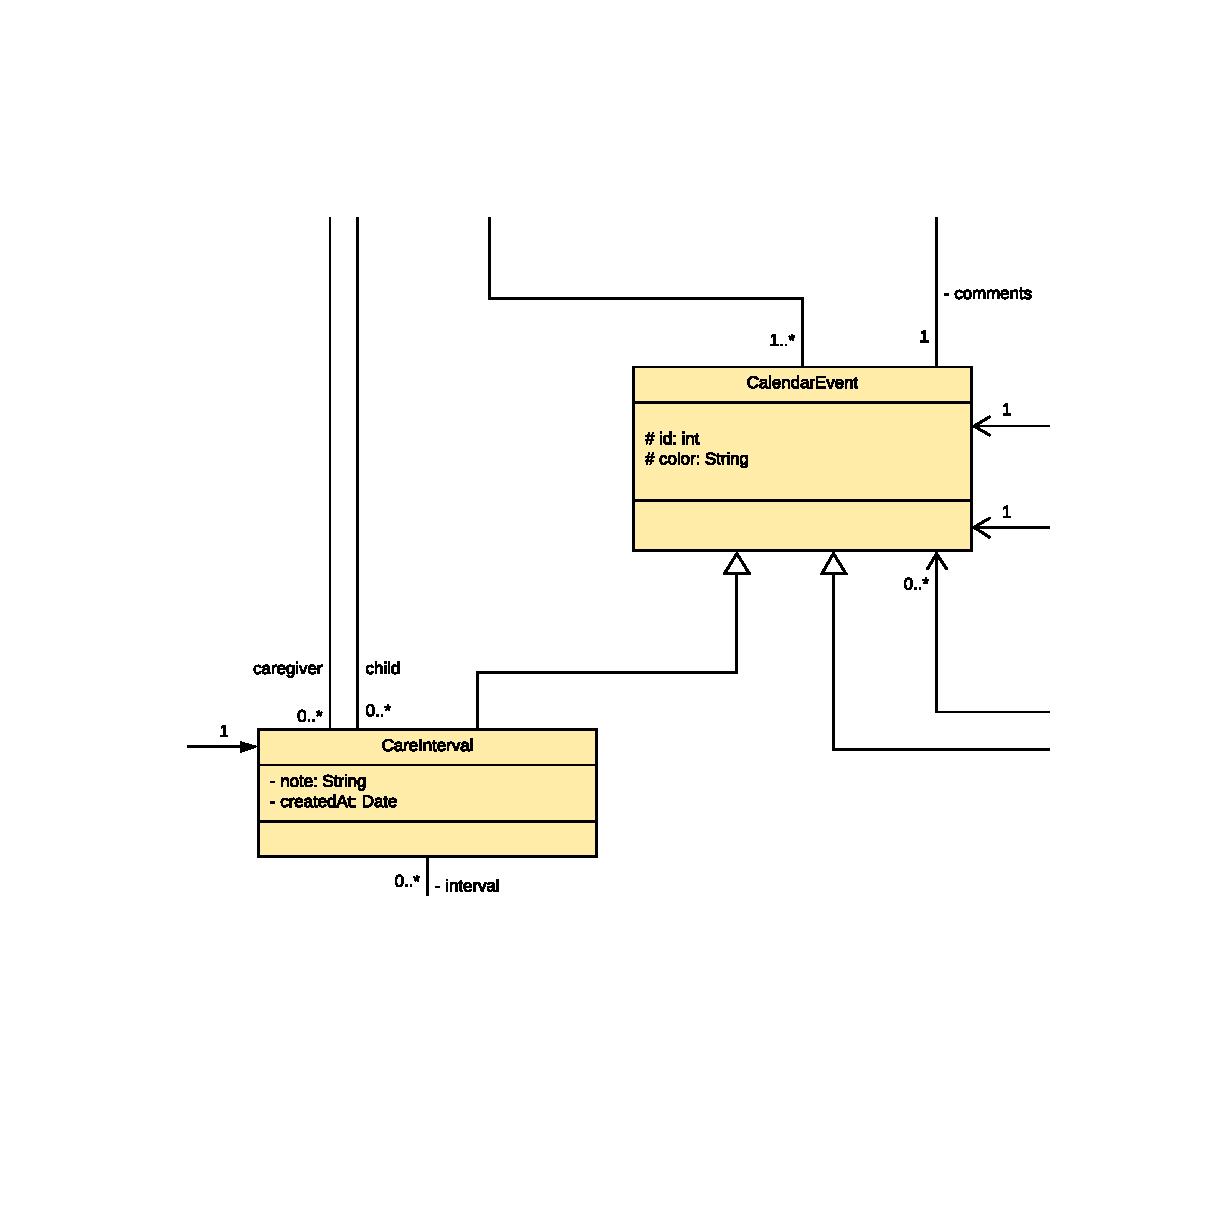
\includegraphics[width=0.7\textwidth]{pdfs/CareDays1}
	            \caption[Návrh pečovatelských dnů]{Návrh pečovatelských dnů podle Doménového modelu předmětu BI-SP2}\label{image:caredays1}
            \end{figure}
            Aktuální návrh pečovatelských dnů je příliš komplikovaně navržen\ref{image:caredays1}. Dlouhodobá nastavení pečovatelských dnů rodičů nevyžaduje komplikovaný návrh intervalů (viz sekci \ref{analyza:pozadavky-frontendu}). Také je potřeba přidat odkaz na konkretního rodiče, který je zodpovědný za tento den pro zjednodušení práce s touto entitou v rámci frontedové části aplikace. Pro návrh jednorázových změn pečovatelských dnů aktuální návrh je vhodnější než pro dlouhodobá pravidla, protože komplikované intervaly jsou vyžadovány. Popis navržených změn a následné implementace bude popsán v sekci \ref{navrh:upravy:caredays}
            
         \subsection{Oznámení}
            \begin{figure}\centering
	            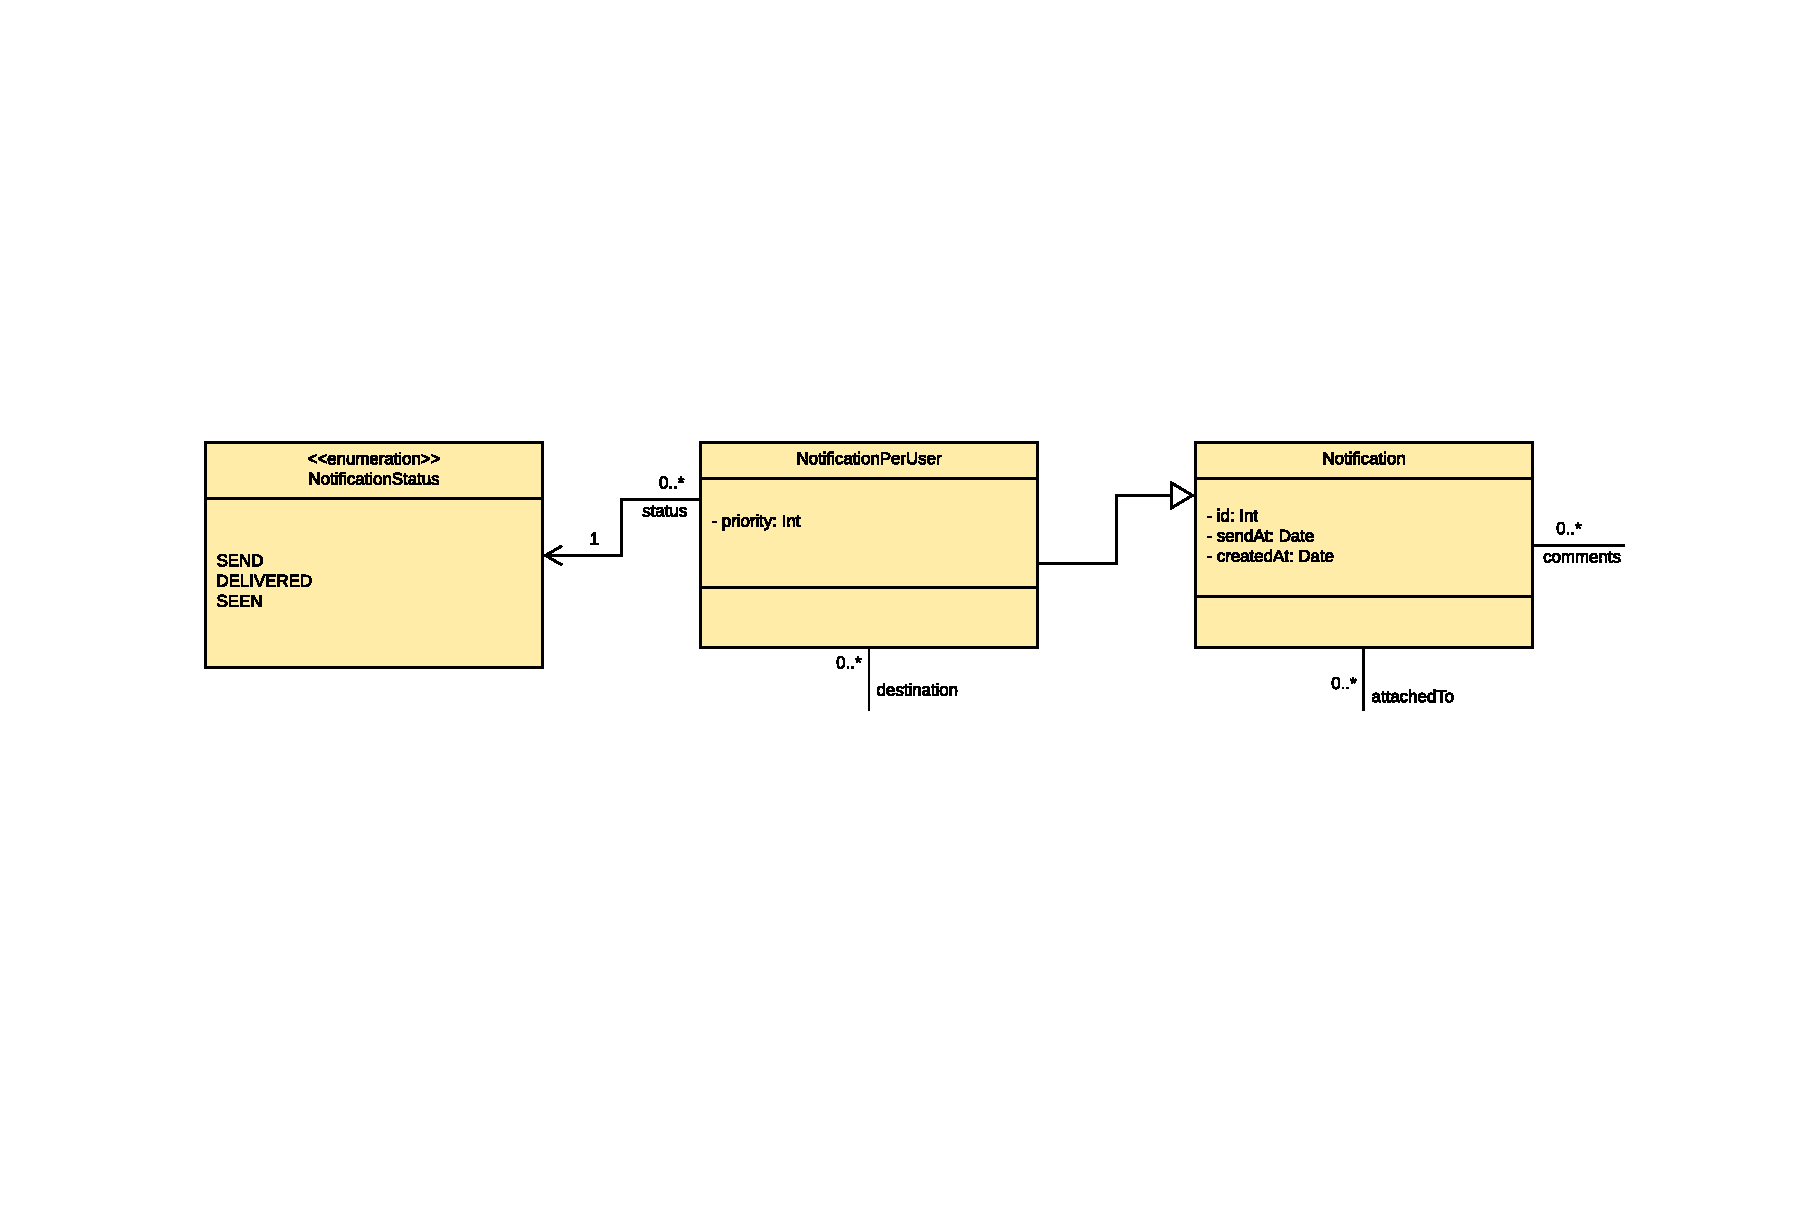
\includegraphics[width=0.8\textwidth]{pdfs/Notification1}
	            \caption[Předchozí návrh oznámení]{Návrh oznámení podle doménového modelu předmětu BI-SP2}\label{image:notification1}
            \end{figure}
            Současný návrh oznámení (viz obrázek \ref{image:notification1}) reprezentují upozornění uživatele o nějakém požadavku na změnu. Příčin oznámení uživatele ve skutečnosti je více:
            \begin{itemize}
                \item změny pečovatelských dnů
                \item alimenty
                \item změny nastavení alimentů
                \item potřeby dítěte
                \item změny v rámci rodiny
            \end{itemize}
            Frontendová část aplikace vyžaduje přizpůsobení oznámení upozorněním v rámci Android aplikace, což vyžaduje úpravu atributů. Také je potřeba specifikovat která událost způsobilá vytvoření tohoto oznámení a přidat typ této události podle výše uvedeného seznamu. Za účelem navrženi kvalitnějšího API také je potřeba přidat možnost přečíst všechny upozornění, které má uživatel, najednou. Řešení problému bude popsáno v sekci \ref{navrh:upravy:notification} . 
            
            % reprezentuje libovolný typ oznámení. Tudíž oznámení pomocí elektronické pošty a pomocí upozornění v telefonu jsou reprezentovány pomocí stejné entity.
            
            % Frontedová část aplikace vyžaduje přizpůsobení oznámení upozorněním v rámci Android aplikace, což je konkretním typem oznámení a vyžadují sadu specifických atributu:
            % \begin{itemize}
            %     \item ID
            %     \item 
            % \end{itemize}
            % Řešení tohoto problému bude popsáno v sekci \ref{navrh:upravy:notification}
            
    % \section{Analýza konkurence}
    %     Tento návrh...
% \section{Analýza testování}

\section{Analýza bezpečnosti}
    
    \subsection{Role}\label{analyza:bezpecnost:role}
    
    % Aplikace je navržená tak, že první věc, kterou uživatel udělat, je registrace. Uživatel potřebuje zvolit jméno, příjmení, email a heslo. Na základě těchto údajů se vytváří účet uživatele. V Doménovém modelu tato třída se jmenuje \texttt{User}. V tento okamžik uživatel má role \texttt{USER}, která mu nadává možnost udělat jenom omezený počet věcí.  
        Než se uživatel přihlásí do rodiny, nemá žádnou roli nebo má roli uživatele bez rodiny. V takovém stavu uživatel by měl mít velice omezena přístupová práva. 
        
        \begin{figure}\centering
	        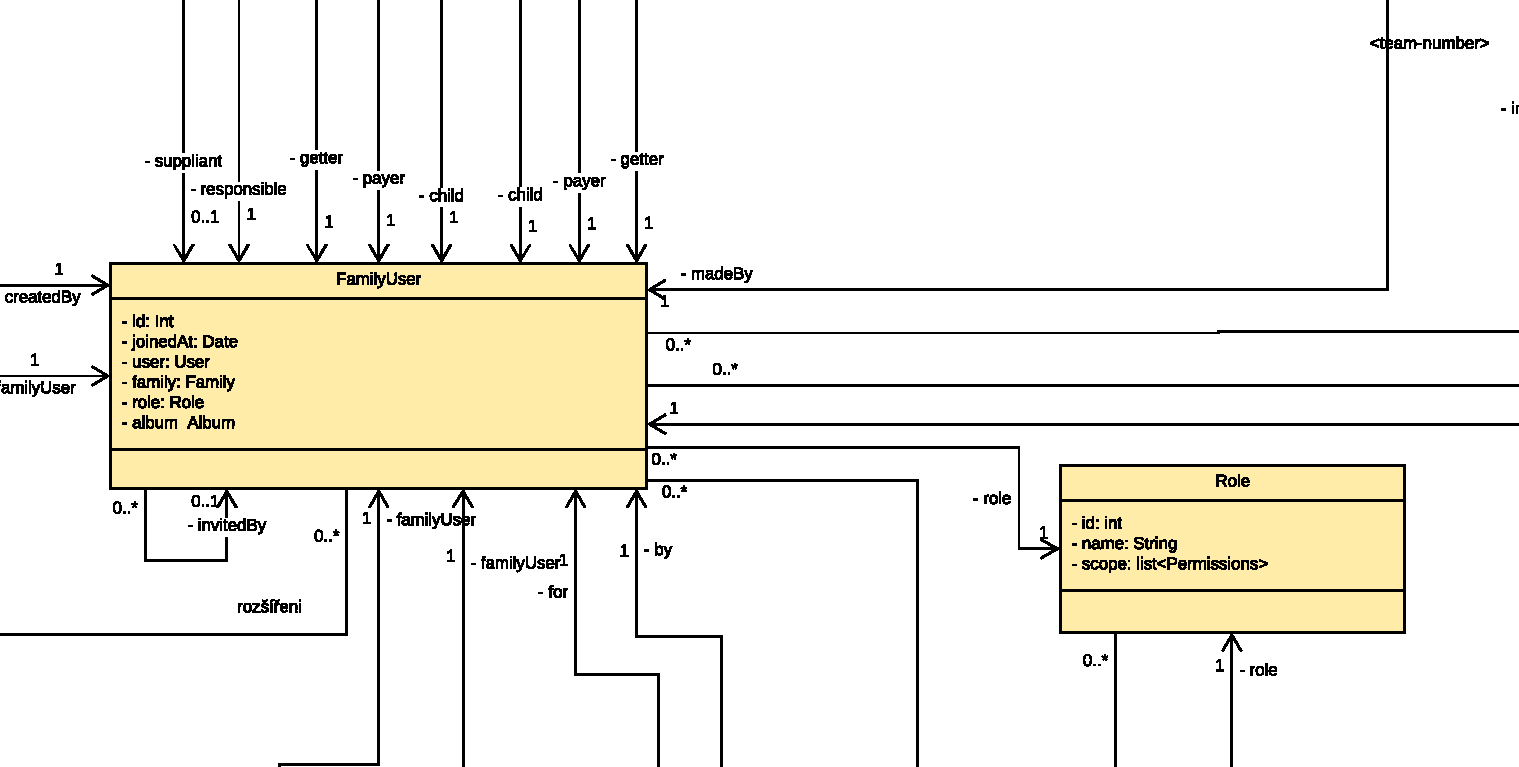
\includegraphics[width=1.0\textwidth]{pdfs/Role1}
	        \caption[Návrh \texttt{Role}]{Návrh entity \texttt{Role} podle Doménového modelu z předmětu BI-SP2}\label{image:Role1}
        \end{figure}
        Po přihlášeni do rodiny uživatel má svou vlastní roli (viz obrázek \ref{image:Role1}), podle které mohou lišit jeho přístupová práva. Hlavní rolí v aplikace je rodič. Uživatel s takovou rolí má přístup ke všem potřebám dítěte a všem záznamem v kalendáři. Také, rodič může vytvořit pozvání do rodiny pro libovolného uživatele a nastavit mu libovolnou roli, včetně roli rodiče. Mimořádnou roli v rámci systému je dítěte. Uživatel s takovou rolí nemůže vlastnit pečovatelský den nebo splnit přání. Přihlášení dítěte muže proběhnout i bez vytvořeni klasického uživatele systému. Ostatní uživatele v rodině mají roli příbuzného.
    
    \subsection{Autorizace}
        Návrh bezpečné aplikace nebyl cílem předmětu zmíněných v sekcích \ref{analyza:navrh:sp1} a \ref{analyza:navrh:sp2}. Proto návrh a současná implementace neobsahuje proces přihlašovaní uživatele do systému. Nový procesu přihlašovaní bude zmíněn v sekci \ref{navrh:bezpecnost}.
        
\section{Analýza testování}\label{analyza:testovani}
    Současný návrh neobsahuje informaci o implementaci testování. Současná implementace obsahuje jednu třídu, obsahující test, který se zaměřuje na ověření, zda se načetl {kontext aplikace}\footnote{Pokročilý kontejner, který funguje podobně \texttt{BeanFactory}. Načítá definice beanů, provazuje je a vydává v případe nutnosti} (viz obrázek \ref{code:test-context-loads1}).
    \begin{figure}
    \begin{minted}{java}
@RunWith(SpringRunner::class)
@SpringBootTest
class RozvodyApplicationTests {

    @Test
    fun contextLoads() {
    }

}
        \end{minted}
        \caption{Ukázka současného testování} 
        \label{code:test-context-loads1}
        \end{figure}
\section{Průběžná integrace}
    TODO CI
   